\documentclass[12pt,a4paper,twoside]{book}


\usepackage[utf8]{inputenc}
\usepackage[a4paper,inner=3.5cm,outer=2.5cm]{geometry}

\usepackage[titletoc,title,toc,page]{appendix}
\usepackage{verbatim}
\usepackage{placeins}
\usepackage{listings}
\usepackage{hyperref}
\usepackage[italian]{babel}
\usepackage{tikz}
\usepackage{parskip}

\usepackage{graphicx}
\usepackage{blindtext}
\usepackage{chngcntr}
\counterwithin{table}{chapter}

\usepackage{newlfont}
\usepackage{fancyhdr}
\usepackage{indentfirst}
\usepackage[utf8]{inputenc}
\usepackage{float}
\usepackage{hyperref}
\usepackage[capitalize,noabbrev]{cleveref}
\usepackage{soul}
\usepackage[font=footnotesize,labelfont=bf]{caption}

\usepackage{multirow}
\usepackage{hyphenat}
\hyphenation{mate-mati-ca recu-perare}

\usepackage{lscape} 

\usepackage{natbib}
\bibliographystyle{alpha}
\setcitestyle{super,open={[},close={]}}

\newcommand{\rom}[1]{\uppercase\expandafter{\romannumeral #1\relax}}

\usepackage{pdfpages}

\begin{document}
% Per spostare i vari elementi più su o più giù gioca con i valori di vspace che ci sono tra uno e l'altro
\pagestyle{empty}
\newgeometry{
    left=20mm,
    right=20mm,
    top=20mm,
    bottom=20mm
}

\begin{titlepage}

\begin{center}

% marchio di ateneo

\includegraphics[width=6.5cm,height=4.7cm]{img/logo/marchio-di-ateneo.png}

\vspace{10mm}

% \large is 12pt
{\large{\bf{Dipartimento di }}} 

\vspace{5mm}

% \Large is 14.4pt
{\Large{\bf{Corso di Laurea in }}}

\vspace{15mm}

{\Huge{\bf Titolo della tesi }}\\
\vspace{3mm}
{\Huge{\bf anche su più}}\\
\vspace{3mm}
{\Huge{\bf righe }}\\
\vspace{3mm}

\end{center}

\vspace{10mm}

\begin{minipage}[t]{0.40\textwidth}
{\Large{\bf Relatore: \\ Chiar.mo Prof.\\ Nome Cognome}}

\vspace{3mm}

{\Large{\bf Correlatore: \\ Chiar.mo Prof.\\ Nome Cognome}}
\end{minipage}
\hfill
\begin{minipage}[t]{0.40\textwidth}\raggedleft
{\Large{\bf Presentata da: \\ Nome Cognome}}
\end{minipage}

\vspace{30mm}

\rule[0.5cm]{15.8cm}{0.6mm}

\begin{center}
{\large{\bf Sessione mese anno \\}}
{\large{\bf Anno Accademico 20xx/20xx\\}}
\end{center}

\end{titlepage}

\restoregeometry
\newpage
\begin{center}
    (DA FARE ALLA FINE)\\
    5 parole chiave per caratterizzare il contenuto della dissertazione:\\ (se non ti piacciono così sparse puoi anche semplicamente scriverle su una riga sola)
\end{center}

% https://tex.stackexchange.com/questions/26538/words-scattered-randomly-in-on-coverpage
\begin{tikzpicture}[overlay,remember picture,shift=(current page.center)]
\pgfmathsetseed{3}


\foreach [count=\count] \word in {Parola 1, parola 2, parola 3, parola 4, parola 5} {
\node [
    xshift={(mod(\count,3)-1)*(\paperwidth/4)},
    yshift={(mod(\count,7)-3)*(\paperwidth/6)},
    xshift=rand*4cm,
    yshift=rand*2cm,
    % rotate=rand*35,
    % opacity=rnd*0.5+0.125,
    font=\large] {\word};
}
\end{tikzpicture}
\newpage

\topmargin=6.5cm
\begin{flushright}
\emph{
\LARGE{La dedica}\\\vspace{2mm}
\LARGE{anche quella se vuoi}\\\vspace{3mm} 
\LARGE{su più righe} 
}
\end{flushright}
\newpage~\newpage
\pagenumbering{gobble}
\chapter*{Abstract}
Abstract qui (ti consiglio di farlo alla fine)

\topmargin=-1cm
\tableofcontents
\thispagestyle{empty}
\listoftables
\thispagestyle{empty}
\listoffigures
\thispagestyle{empty}
\newpage~\newpage


% \pagenumbering{arabic}
% \setcounter{chapter}{-1}
% \raggedbottom
% \chapter{INTRODUZIONE} \label{chap:intro}
% \pagestyle{plain}
% \setcounter{page}{1}


%%%%%%%%%%%%%%%%%%%%%%%%%%%%%%%%%%%%%%%%%%%%%%%%%%%%%%%%%%
% Acoustics and Music Technology Final Project Latex Template
%
% CHAPTER 1 PAGE
%
% TOTAL EDITS REQUIRED: 1
%
% NOTE: NO NEED TO INCLUDE ANY FURTHER PREAMBLE IN THIS FILE
%%%%%%%%%%%%%%%%%%%%%%%%%%%%%%%%%%%%%%%%%%%%%%%%%%%%%%%%%%


%%%%%%%%%%%% EDIT %%%%%%%%%%%%
\chapter{Solving the Problem of Digital Conservation of Musical Instruments}
\label{chapter1}

\section{Open Science}

\subsection{Sustainable Software Engineering}

\section{Digital Conservation}

\subsection{Musical Instruments and Digital Cultural Heritage}

\section{Thesis Structure}

%%%%%%%%%%%% EDIT %%%%%%%%%%%%

%%%%%%%%%%%%%%%%%%%%%%%%%%%%%%%%%%%%%%%%%%%%%%%%%%%%%%%%%%
% Acoustics and Music Technology Final Project Latex Template
%
% CHAPTER 2 PAGE
%
% TOTAL EDITS REQUIRED: 1
%
% NOTE: NO NEED TO INCLUDE ANY FURTHER PREAMBLE IN THIS FILE
%%%%%%%%%%%%%%%%%%%%%%%%%%%%%%%%%%%%%%%%%%%%%%%%%%%%%%%%%%


%%%%%%%%%%%% EDIT %%%%%%%%%%%%
\chapter{Finite Difference Time Domain}
\label{chapter2}
%%%REVISE THIS SECTION
The finite-difference time-domain method is a technique which is considered to be one of the most intuitive and simplest ways to approximate a continuous variable function \textit{u(t)} (Bilbao/Schneider) by time series. To approximate this continuous function we say that $u(t_{n})=u(nk)$ for integer $n$, where \textit{k} is considered to be the time step between each value in the time series.\\
In regard to musical applications, these technique yields very interesting and accurate results. This is due to the fact that, as for most audio applications the step time is relatively small. Considering that in audio, the sampling rate is standarized to normally about 44100 Hz, we can see how this time step $k=1/Fs$, will be small enough so that information is preserved with a good degree of accuracy. 

\section{Difference operators}
\label{chapter2:sec1}
In order to produce an approximation to a continuous function through a time series, it is necessary to define a series of operators that are applied to the the approximation. In this case, the operators that are necessary to simulate the function at a particular time will involve different time steps of the approximating series. Therefore for a time series ${u}^{n}$ where $n$ represents the $n^{th}$ time step, it is necessary to introduce the following 
\begin{equation*}
	e_{t+}u^{n} = u^{n+1}  \ \ \ \ \ \  e_{t-}u^{n} = u^{n-1}    \ \ \ \ \       $ e_{t+}e_{t-} = 1
\end{equation*}
These operators are defined as forward and backwards shifts respectively. Thanks to these operators, it is possible to approximate a wide variety of continuous operators, although for the purposes of this paper they will be limited to approximate first and second derivatives.
To produce an approximation to the first derivative operator, it is possible to use different combinations of the backward and forward shifts as follows,
\begin{equation}
	\begin{aligned}
	\delta_{t+} \overset{\Delta}{=} \frac{1}{k} (e_{t+} -1) \cong \frac{d}{dt}
	\end{aligned}
\end{equation}
\begin{equation}
	\begin{aligned}
	\delta_{t-} \overset{\Delta}{=} \frac{1}{k} (1 - e_{t-}) \cong \frac{d}{dt}	
	\end{aligned}
\end{equation}
\begin{equation}
	\begin{aligned}
	\delta_{t\cdot} \overset{\Delta}{=}  \frac{1}{2k} (e_{t+} -e_{t-}) \cong \frac{d}{dt}
	\end{aligned}
\end{equation}
These operators are defined as forward, backward, and centered difference operator respectively.\\ 
It is possible to extend this techinique to higher order derivatives, like for example second order derivatives. To do so, we will require the product of two of the previous difference operators. Hence, the second order difference operator \textit{$\delta_{tt}$} is defined by
\begin{equation}
\label{eqn:ddiff}
	\begin{aligned}
	\delta_{tt} \overset{\Delta}{=} \delta_{t+}\delta_{t-}=\frac{1}{k^2}(e_{t+}-2+e_{t-})\cong\frac{d^2}{dt^2}
	\end{aligned}
\end{equation}  
The reader at this point might have already realized the possibility of combining difference operators to for example approximate second order partial derivatives, this approximation consists on the product of two difference operators acting on different variables. As an example, we will consider the approximation to the double partial derivative $\frac{\partial^{2}}{\partial x \partial y}$,
\begin{equation}
	\begin{aligned}
	\delta_{x+}\delta_{y-}  \overset{\Delta}{=} \frac{1}{k^2} (e_{x+} -1) (1-e_{y-} )=\\
		=\frac{1}{k^2}(e_{x+}-e_{x+}e_{y-}-1+e_{y-}) \cong  \frac{\partial^2}{\partial x \partial y}
	\end{aligned}
\end{equation}


%%%%%%%%%%%% EDIT %%%%%%%%%%%%
%%%%%%%%%%%%%%%%%%%%%%%%%%%%%%%%%%%%%%%%%%%%%%%%%%%%%%%%%%
% Acoustics and Music Technology Final Project Latex Template
%
% CHAPTER 3 PAGE
%
% TOTAL EDITS REQUIRED: 1
%
% NOTE: NO NEED TO INCLUDE ANY FURTHER PREAMBLE IN THIS FILE
%%%%%%%%%%%%%%%%%%%%%%%%%%%%%%%%%%%%%%%%%%%%%%%%%%%%%%%%%%

\chapter{Analysis: Magpie}\label{analysis-magpie}

\section{The Problem}\label{the-problem-2}

\subsection{Plate Theory}\label{plate-theory}

\subsection{Boundary Conditions}\label{boundary-conditions}

\section{The Solution}\label{the-solution-1}

\subsection{Implementation}\label{implementation}

\subsubsection{Discretising}\label{discretising}
\subsubsection{Design}\label{design}

\section{Application}\label{application-1}
%%%%%%%%%%%% EDIT %%%%%%%%%%%%

\chapter{2D wave equation}
\label{chapter3}
\section{2D wave equation}
\label{chapter3:sec1}
The discussion of this chapter will be mainly focused on the wave equation. This simple second order partial differential equation describes the motion of waves over a domain \textit{D}. It is defined as follows,
\begin{equation}
\label{eqn:wave}
	u_{tt}=c^{2}\nabla u
\end{equation} 
Where $u_{tt}$ represents the second order partial derivative with respect to time $t$, $c$ is the wave speed and $\nabla u$ represent the Laplacian operator over $u$. Before the study on the wave equation continuous it is necessary to define the Laplacian operator.\\
The Laplacian operator $\nabla$ can operate on $u$ on different dimensions dependent of the variables affecting $u$. If we consider for example $u$ to be a 3D vector, we can describe the Lapalacian operation on $u$ by the following equation
\begin{equation}
	\nabla u = \frac{\partial^2}{\partial xx}u + \frac{\partial^{2}}{\partial yy}u + \frac{\partial^{2}}{\partial zz}
\end{equation}
Thus, if we want to operate in lower dimensions say 1D or 2D, it will only be necessary to define the operator over 1 or 2 variables resprectively.\\
It is possible now to rearrange Eq.\ref{eqn:wave} for a two dimensional domain \textit{D} to achieve the equation,
\begin{equation}
	u_{tt}=c^{2}( \frac{\partial^2}{\partial xx}u + \frac{\partial^{2}}{\partial yy}u)	
\end{equation}
 If we consider \textit{D} to be of finite dimension, we can rearrange the above expression as
\begin{equation}
\label{eqn:wave2}
	\begin{aligned}
	u_{tt}=\gamma^{2}(\frac{\partial^2}{\partial xx}u + \frac{\partial^{2}}{\partial yy}u)
	\end{aligned}
\end{equation}
Where $\gamma=c/L$ and $L=\sqrt{|D|}$.\\
\subsection{Exact solution and analysis}
\label{chapter3:sec1:ssec1}
This particular kind of PDE admits an exact solution of the form $u(x,y,t)=\e^{st+j(\beta_{x}x+\beta_{y}y)}$, therefore, if we introduce this solution into \ref{eqn:wave2}, this yields,
\begin{equation}
		s^{2}=-\gamma^{2}(\beta_{x}^{2}+\beta_{y}^{2})
\end{equation}
From which we can reach the dispersion relation,
\begin{equation}
	\begin{aligned}
	\omega=\pm \gamma|\mathrm{\beta}| \ \ \ \ \     \text{where} \ \ \ \ \     |\mathrm{\beta}|=\sqrt{(\beta_{x}^{2}+\beta_{y}^{2})}
	\end{aligned}
\end{equation}
And so we can derive the expressions for phase and group velocity $\textit{v}_{\phi}$ and $\textit{v}_{g}$
\begin{equation}
	\begin{aligned*}
		\textit{v}_{\phi}&=\frac{\omega}{\mathrm{\beta}}&=\gamma \ \  
		\textit{v}_{g}&=\frac{\partial \omega}{\partial\mathrm{\beta}}&=\gamma
	\end{aligned*}
\end{equation}
We can see by the above equations that all the waves will travel at the same speed independently of frequency and wavenumber. This kind of behaviour is defined as $\textit{nondispersive}$.
\subsection{Initial and boundary conditions}
\label{chapter3:sec1:ssec2}
In order to initialise this PDE, it is necessary to define a set of initial conditions. These are normally defined by an initial displacement $u(x,y,0)=u_{0}(x,y)$ and an initial velocity $(\partia u/ \partial t)=v_{0}(x,y)$ but for purposes of this paper this set of initial conditions are not required given that the wave equation will be driven by force $f(t)$.\\ 
Considering the fact that this wave propagation is produced over a finite domain, it is necessary to introduce a set of conditions to determine the different behaviour at the boundaries.\\
Two typical conditions are defined by the following equations
\begin{equation}
	u(0,y,t)=0 \\\\\ u_{x}(0,y,t)=0
\end{equation}
Which are refered as Dirichlet and Neumann conditions respectively. The former will represent the behaviour of the boundaries when this are fixed while the later will represent a fixed behaviour. For purposes of this paper, we will consider that the boundaries of our domain behave under Dirichlet conditions, this is due to the simplicity of imposing such condition.
\section{2D wave equation using FDTD}
\label{chapter3:sec1}
The study will continue by approximating the above equations using FDTD schemes. There are different ways of approximating this equation depending on the approximation to the Laplace operator. This paper will cover two ways of approximating $\nabla$ in cartesian coordinates, a five point approximation and a nine point approximation.
\subsection{Five point approximation}
\label{chapter3:sec1:ssec1}
One way to approximate the 2D Laplacian operator is to use a five point stencil. By a five point stencil, we refer to the fact that to produce an approximation to $\nabla$ at a particular point $u_{(x,y)}^{n}$, we will take in consideration two neighbouring points of $u_{(x,y)}^{n}$ with respect to each coordinate.\\
If we consider that $\frac{\partial^{2}}{\partial xx}\cong\delta_{xx}$ as define in Eq.\ref{eqn:ddiff} we can defined $\delta_{\delta\boxplus}$ as
\begin{equation}
	\delta_{\delta\boxplus}=\delta_{xx}+\delta{yy}\cong \Delta
\end{equation}
Equation \ref{eqn:wave2} can therefore be expressed as follows
\begin{equation}
	\delta_{tt}u=\gamma^{2}\delta_{\Delta\boxplus}u
\end{equation}
\begin{figure}[tb!]
\begin{center}
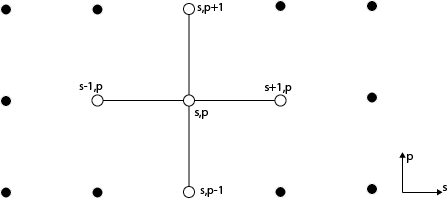
\includegraphics[width=10cm]{./Chapter_3/_Figs/5point.png}
\caption{Five point stencil for a given point at location (s,p) in a two dimensional grid.}
\label{figs:5point}
\end{center}
\end{figure}
Where $u=u^{n}_{x,y}$  which represent a two dimensional grid where each point is represented by a particula choice of integers $x$ and $y$. $x$ and $y$ in this case will represent the approximation to the points $x=xh_{x}$ and $y=yh_{y}$ where $h_{x}$ and $h_{y}$ represent the grid spacing on the $X$ and $Y$ coordinates resprectively. For simplicity in this paper, we will consider an equally spaced grid, thus $h=h_{x}=h_{y}$.\\
Expanding the above expression we yield the following equation
\begin{equation}
	\frac{1}{k^2}(u^{n+1}_{x,y}-2u^{n}_{x,y}+u^{n-1}_{x,y}=\gamma^{2}\frac{1}{h^2}((u^{n}_{x+1,y}-2u^{n}_{x,y}+u^{n}_{x-1,y})+(u^{n}_{x,y+1}-2u^{n}_{x,y}+u^{n}_{x,y-1}))\\
\end{equation}
Which can be rearranged to
\begin{equation}
\label{eqn:FD5wave}
	u^{n+1}_{x,y}=2u^{n}_{x,y}-u^{n-1}_{x,y}+\lambda^{2}(u^{n}_{x+1,y}+u^{n}_{x-1,y}+u^{n}_{x,y+1}+u^{n}_{x,y-1}-4u^{n}_{x,y})
\end{equation}
For $\lambda=\frac{k\gamma}{h}$.\\
It is worth noting that there is a condition that must be impossed to $\lambda$ so that the solution is stable. This condition is developed by using Von Neumann analysis on \ref{eqn:FD5wave} using the solution $u^{n}_{s,p}=z^{n}\e^{jh(s\beta_{x}+p\beta_{y}})$ and solving for $z$. Since $z$ must satisfy to be unit modulus,$\lambda$ must satisfy $\lambda\leq \frac{1}{\sqrt{2}}$ (for further explanation see Bilbao).
\subsection{Nine point approximation}
\label{chapter3:sec1:ssec2}

In order to get a more accurate approximation, we can use stencils with a higher number of points, say a nine point interpolation. This kind of method will require a higher computational cost but it will increase the level of nondispersivity of the model with respect to the five point stencil approximation.
In order to develope the nine point approximation we will need to define first another type of operator represented by $\delta_{\Delta\boxtimes}$ which is defined by
\begin{equation}
	\delta_{\Delta\boxtimes}=\delta_{xx}+\delta_{yy} +\frac{h^2}{2}\delta_{xx}\delta_{yy}
\end{equation}
This leads to
\begin{equation}
	\delta_{tt}u=\gamma^{2}(\alpha\delta_{\Delta\boxplus} u + (1-\alpha)\delta_{\Delta\boxtimes}u)
\end {equation}
Which can be rearranged using similar techiniques of Eq.\ref{eqn:FD5wave} to
\begin{figure}[tb!]
\begin{center}
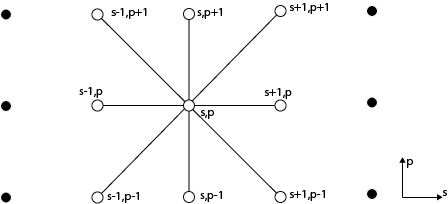
\includegraphics[width=10cm]{./Chapter_3/_Figs/9point.png}
\caption{Nine point stencil for a given point at location (s,p) in a two dimensional grid.}
\label{figs:9point}
\end{center}
\end{figure}
\begin{equation}
\label{eqn:FD9wave}
	\begin{align}
		u^{n+1}_{s,p}&=2u^{n}_{x,y}-u^{n-1}_{x,y}+\lamba^{2}(u^{n}_{x+1,y}+u^{n}_{x-1,y}+u^{n}_{x,y+1}+u^{n}_{x,y-1}-4u^{n}_{x,y}\\
				    &+(\frac{1}{2}(1-\alpha))(u^{n}_{x+1,y+1}+u^{n}_{x+1,y-1}+u^{n}_{x-1,y+1}+u^{n}_{x-1,y-1}\\
				    & -2(u^{n}_{x+1,y}+u^{n}_{x-1,y}+u^{n}_{x,y+1}+u^{n}_{x,y-1})+4u^{n}_{x,y} )
	\end{align}
\end{equation}
Once again if we apply von Neumann analysis to the above expression, we will yield a stability condition on $\lambda$ which is,
\begin{equation}
	\alpha \geq 0  \ \ \ \ \text{and} \ \ \ \ \    \lambda\leq min(1,\frac{1}{\sqrt{2\alpha}}) 
\end{equation}
After some analysis on the accuracy of nine point approximation, results show a better nondispersive behaivour when $\alpha$ sits between the values of 0.6 and 0.8.(Bilbao).\\
It is also worth noting the fact that for $\alpha=1$ this kind of approximation will result in a five point approximation. It can be therefore considered as the general formula for both kinds of approximations.\\

%%%%%%%%%%%% EDIT %%%%%%%%%%%%
%%%%%%%%%%%%%%%%%%%%%%%%%%%%%%%%%%%%%%%%%%%%%%%%%%%%%%%%%%
% Acoustics and Music Technology Final Project Latex Template
%
% CHAPTER 4 PAGE
%
% TOTAL EDITS REQUIRED: 1
%
% NOTE: NO NEED TO INCLUDE ANY FURTHER PREAMBLE IN THIS FILE
%%%%%%%%%%%%%%%%%%%%%%%%%%%%%%%%%%%%%%%%%%%%%%%%%%%%%%%%%%


%%%%%%%%%%%% EDIT %%%%%%%%%%%%
\chapter{Radiation from vibrating bodies}
\label{chapter4}
The following chapter will study the different behaviour and models of sound generation depending on the source of choice.\\
Before we go into the study of the different behaviours, it is necessary to understand what an acoustical source. In Springer [] a source is defined as any object that generates an acoustical wave. There are various different patterns of wave propagation which are determined by various different parameters. In this study, as previously mention, we will focus on the wave propagation patterns produced by acoustical monopoles, dipoles and quadrupoles. These three acoustical sources can be used to simulate various acoustical objects. For example, a small mounted loudspeaker at low frequency can be considered to radiate sound in an omnidirectional pattern and therefore, it can be simulated by a monopole. In the case of an unmounted loudspeaker, its behaviour resembles more the pattern produced by a dipole, and therefore, can be studied using a dipole approximation. Finally, a quadrupole approximation could be worth of considering when studying tuning forks or perhaps a loudspeaker system.\\
The subsections ahead will give a more detailed explanation of these bodies, paying particular attention to the approximation methods used to simulate its behaivour.
\section{Monopole}
\label{chapter4:sec1}
In order to understand what a monopole source is, let us consider first a small pulsating sphere. If we consider the radius of this sphere to be considerably smaller than the wavelength of the radiated sound, we can consider this object to be a point source. Now, since the sphere is symmetric, every pulse will radiate sound equally in all directions and it is therefore omnidirectional. We define a monopole source as any omnidirectional source whose radius is considered smaller with respect to the wavelength of the sound produced.\\
For the interest of the study, we will only define the monopole once it is introduced into the 2D wave equation.( For a more in depth treatment please refer to [ ].) The introduction of the monopole term into the equation can be considered as the driving force of the system which is now governed by the following equation
\begin{equation}
\label{eqn:Monopole}
	u_{tt}=\gamma^{2}(\Delta u) + f(t)*Q*\delta(x-x_{s}),\delta(y-y_{s})
\end{equation}
Where $\delta(x-x_{s})$ is the dirac delta function on the $x$ coordinate (similarly for  $\delta(y-y_{s})$) $Q$ is the $\textit{monopole strength}$ and $f(t)$ is the driving signal. The point $(x_{s},y_{s})$ determines the position of the source.\\
To produce an accurate approximation to this equation without having excesive computational costs, it is necessary to approximate the dirac delta function to a more suited expression. In order to do so, we will use an approximation by the $sinc$ function which once introduced into the $\ref{eqn:monopole}$ yields
\begin{equation}
	u_{tt}=\gamma^{2}(\Delta u)  + Q*f(t)*(\frac{sin(\pi(x-x_{s}))}{\pi(x-x_{s})})(\frac{sin(\pi(y-y_{s}))}{\pi(y-y_{s})})
\end{equation}
Now, if we consider the FDTD expression for the 2D wave equation using the five point stencil, the approximation is given by the following 
\begin{equation}
\label{eqn:FD5mono}
	\begin{aligned}
	u^{n+1}_{s,p}&=2u^{n}_{s,p}-u^{n-1}_{s,p}+\lamba^{2}(u^{n}_{s+1,p}+u^{n}_{s-1,p}+u^{n}_{s,p+1}+u^{n}_{s,p-1}-4u^{n}_{s,p}) \\
			 &+ Q*f(t)*(\frac{sin(\pi(x-x_{s}))}{\pi(x-x_{s})},\frac{sin(\pi(y-y_{s}))}{\pi(y-y_{s})})
	\end{aligned}
\end{equation}
The above expression produces an approximation illustrated on Figure $\ref{figs:monopole}$. This figure represents the approximation at different time steps of the simulation for a square room of 10 meters of length where the sampling rate of the simulation is 8000Hz. The driving signal of the system is a pure sine wave at 160Hz.
\begin{figure}[h]
\label{figs:monopole}
\begin{subfigure}{0.3 \textwidth}
	\centering
	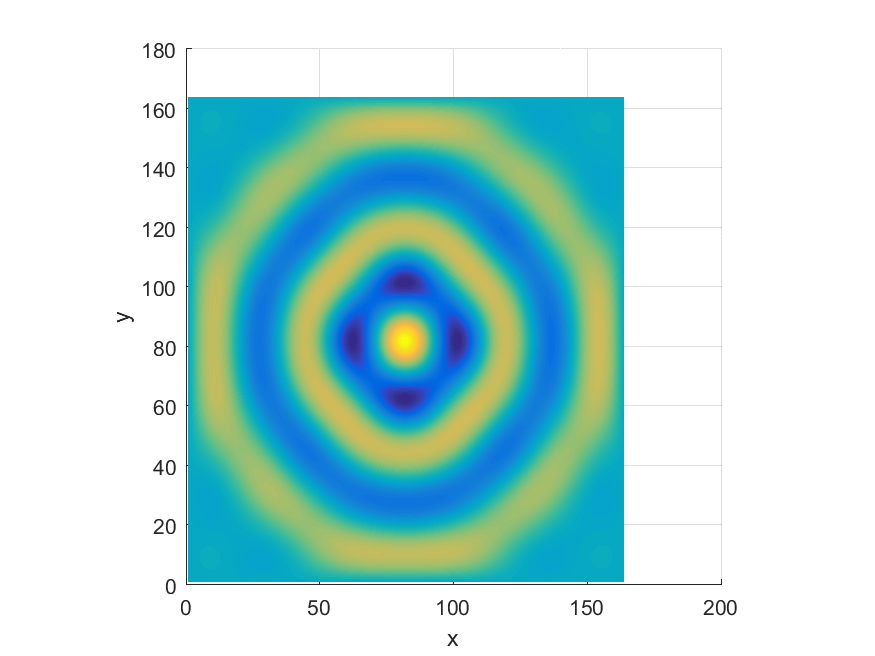
\includegraphics[width=6cm]{../Chapter_4/_Figs/Monopole001_5point_160Hz_L10m_8000Fs.png}
	\caption{T=0.015s}
\end{subfigure}
\begin{subfigure}{0.3 \textwidth}
	\centering
	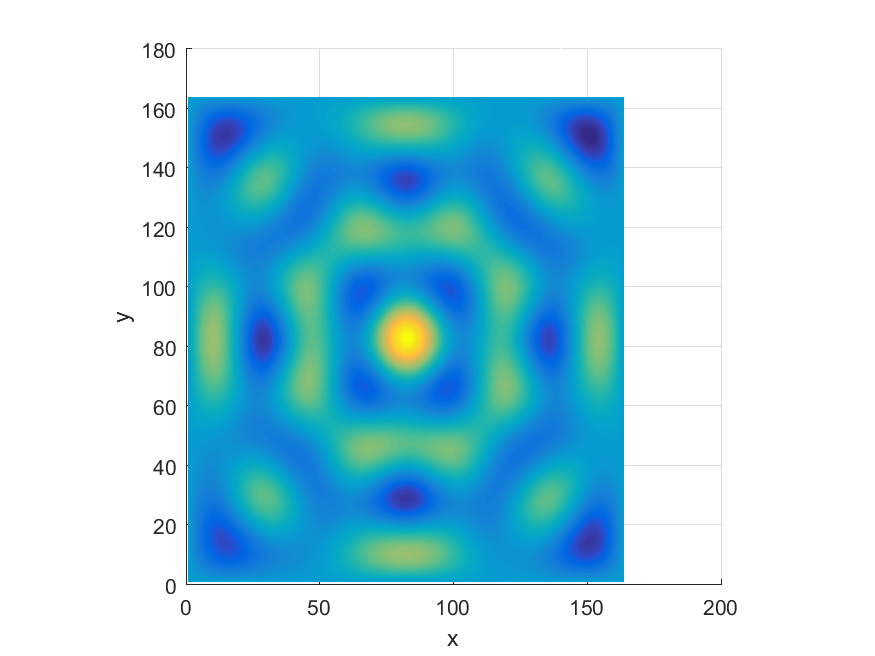
\includegraphics[width=6cm]{../Chapter_4/_Figs/Monopole05_5point_160Hz_L10m_8000Fs.png}
	\caption{T=0.5s}
\end{subfigure}
\begin{subfigure}{0.3 \textwidth}
	\centering
	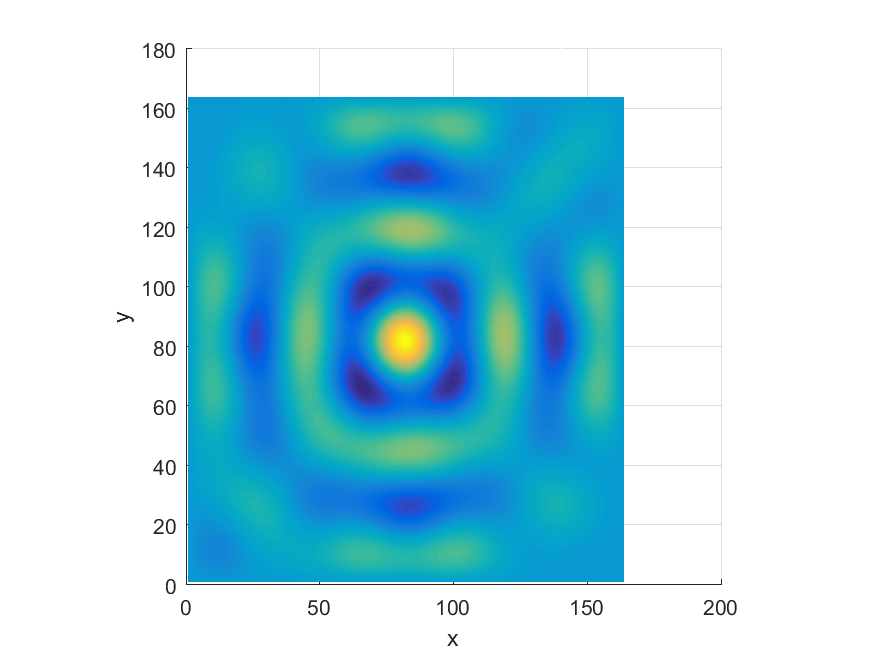
\includegraphics[width=6cm]{../Chapter_4/_Figs/Monopole1_5point_160Hz_L10m_8000Fs.png}
	\caption{T=1s}
\end{subfigure}
\caption{Radiation pattern of monopole approximation at different times T. Produced using 5 point sheme approximation to 2D wave equation}
\end{figure}


\section{Dipole}
\label{chapter4:sec2}
If we consider the combination of out phased monopoles situated in close proximity from one another, the radiation pattern that will be produced is that of a dipole. Moreover, if we reduce the distance between this monopoles to be sufficiently small with respect to the wavenumber, this combination of sources can be considered as a dipole source. Since we can consider a dipole source as a combination of two out phased monopoles, it important to understand the interference between this monopoles, the radiation pattern that a dipole will produce will not be omnidirectional. In fact, there are positions on the space where this combination of radiation will result on the absence of vibration and therefore sound. 
Before we see a clear example of such pattern, let us give a similar treatment to that of the monopole and so, we will only consider the dipole source once it is introduced into the wave equation. Therefore defining a dipole source as the driving force of the following equation we reach the defining expression for such source
\begin{equation}
\label{eqn:Dipole}
	u_{tt}=\gamma^{2}(\Delta u) + f(t)*D*\nabla(\delta(x-x_{s}),\delta(y-y_{s}))
\end{equation}
Since the radiation patterns are not omnidirectional, it is interesting to produce an approximation to the source that can vary its positioning in space and therefore have the possibility of rotation. In order to produce rotation, it is necessary to introduce the following rotation vector $\vec{r}=(cos(\theta),sin(\theta))$, which will multiply the dipole expression and produce a rotation given by the angle $\theta$.\\
Following the analysis of a monopole source, we can reach a similar approximation equation for the wave propagation as
\begin{equation}
\label{eqn:FD5dipo}
	\begin{aligned}
	u^{n+1}_{s,p}&=2u^{n}_{s,p}-u^{n-1}_{s,p}+\lamba^{2}(u^{n}_{s+1,p}+u^{n}_{s-1,p}+u^{n}_{s,p+1}+u^{n}_{s,p-1}-4u^{n}_{s,p}) \\
			&+ Q*f(t)*\vec{r}*\nabla(\frac{sin(\pi(x-x_{s}))}{\pi(x-x_{s})},\frac{sin(\pi(y-y_{s}))}{\pi(y-y_{s})})
	\end{aligned}
\end{equation}
Which produce the radiation patterns illustrated on Figure $\ref{figs:dipole}$ for the same parameters as the ones given for the monopole approximation.
\begin{figure}[h]
\begin{subfigure}{0.3 \textwidth}
	\centering
	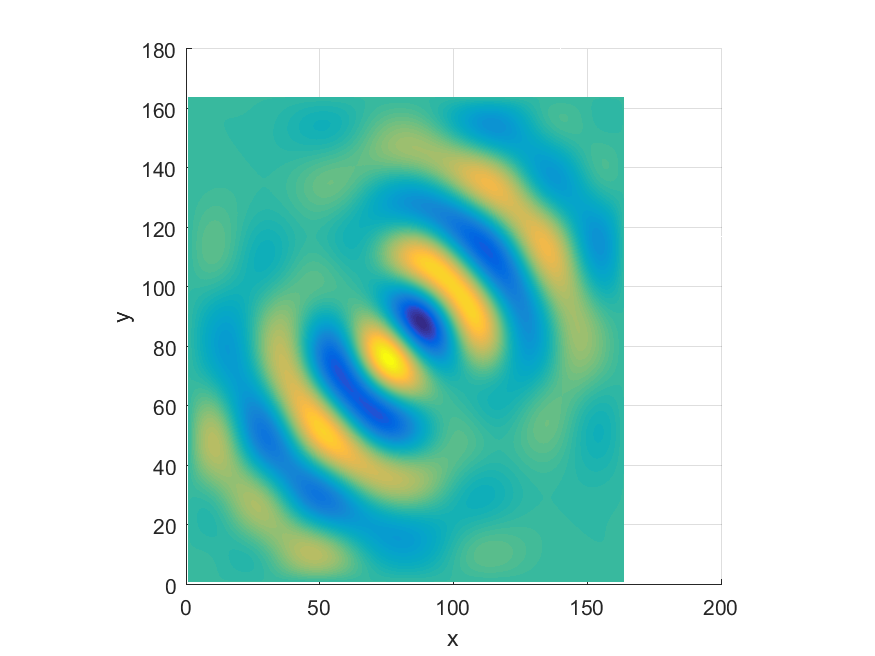
\includegraphics[width=6cm]{../Chapter_4/_Figs/Dipole001_5point_160Hz_L10m_8000Fs.png}
	\caption{T=0.015s}
\end{subfigure}
\begin{subfigure}{0.3 \textwidth}
	\centering
	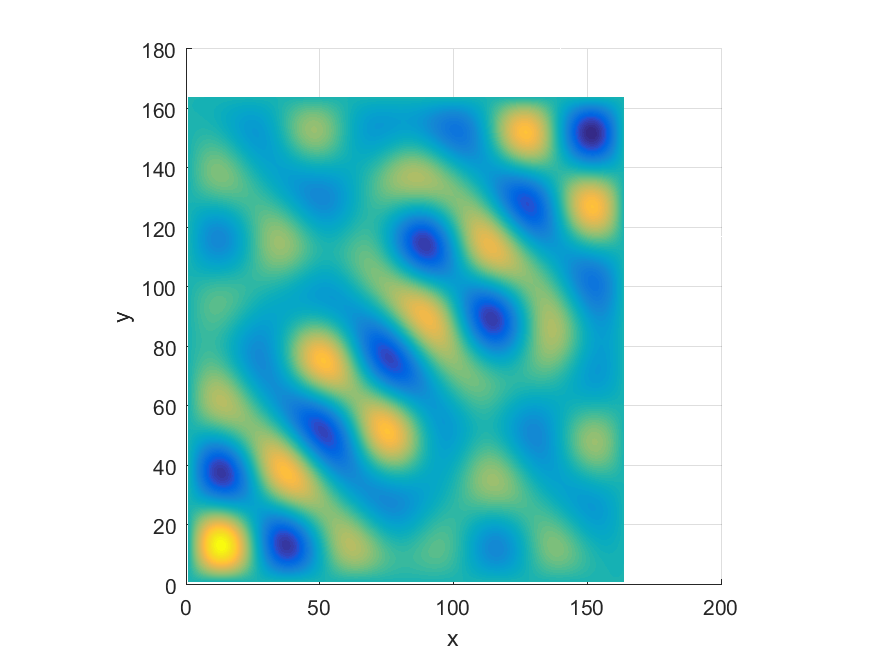
\includegraphics[width=6cm]{../Chapter_4/_Figs/Dipole05_5point_160Hz_L10m_8000Fs.png}
	\caption{T=0.5s}
\end{subfigure}
\begin{subfigure}{0.3 \textwidth}
	\centering
	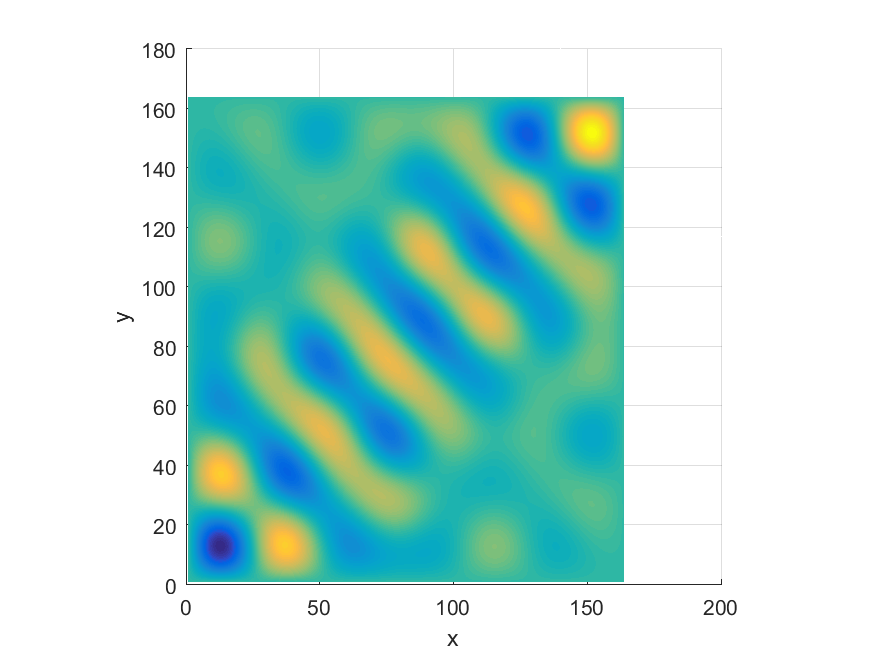
\includegraphics[width=6cm]{../Chapter_4/_Figs/Dipole1_5point_160Hz_L10m_8000Fs.png}
	\caption{T=1s}
\end{subfigure}
\label{figs:dipole}
\end{figure}

\section{Quadrupole}
\label{chapter4:sec3}
The most intuitive way to describe the radiation pattern produced by a quadrupole is to think of it as two dipoles out of phase at a small distance appart. Once again, if this distance is reduced considerably with respect to the wavenumber, this becomes a quadrupole source.\\ 
There are different combination of dipoles that can produce a quadrupole source. In this study, we will focus on two particular quadrupoles, $\textit{lateral}$ and $\textit{longitudinal}$. $\textit{Lateral}$ quadrupole consists on the combination of two perpendicular dipoles while $\texit{longitudinal}$ quadrupole will consists on the combination of two parallel dipoles.\\
Using the previous definition of dipole we can now define the quadrupole as
\begin{equation}
\label{eqn:Quadrupole}
	u_{tt}=\gamma^{2}(\Delta u) + f(t)*C*\nabla^{2}(\delta(x-x_{s}),\delta(y-y_{s}))
\end{equation}
Since the radiation patterns are not omnidirectional, it is interesting to produce an approximation to the source that can vary its positioning in space and therefore have the possibility of rotation. In order to produce rotation, it is necessary to introduce the following rotational matrices respectively for the longitudinal and lateral quadrupole as
\begin{equation}
	Q=\begin{bmatrix}
		cos(\theta)^2   & cos(\theta)sin(\theta)\\
		 cos(\theta)sine(\theta) & sin(\theta)^{2}
	\end{bmatrix}
	\ \ \ \ \
	Q_{x}=\begin{bmatrix}
		cos(\theta)sin(\theta)& 0.5(cos(\theta)^{2}-sin(\theta)^{2})\\
		 0.5(cos(\theta)^{2}-sin(\theta)^{2}) &  cos(\theta)sine(\theta) 
	\end{bmatrix}
\end{equation}  
Which will respectively multiply each particular quadrupole expression and produce a rotation given by the angle $\theta$.\\
Following the analysis of a monopole source, we can reach a similar approximation equation for the wave propagation driven by a lateral quadrupole as
\begin{equation}
\label{eqn:FD5dquadlat}
	\begin{aligned}
	u^{n+1}_{s,p}&=2u^{n}_{s,p}-u^{n-1}_{s,p}+\lamba^{2}(u^{n}_{s+1,p}+u^{n}_{s-1,p}+u^{n}_{s,p+1}+u^{n}_{s,p-1}-4u^{n}_{s,p}) \\
			&+ C*f(t)*Q*\nabla^{2}(\frac{sin(\pi(x-x_{s}))}{\pi(x-x_{s})},\frac{sin(\pi(y-y_{s}))}{\pi(y-y_{s})})
	\end{aligned}
\end{equation}
While the longitudinal quadrupole equation would be given by
\begin{equation}
\label{eqn:FD5dquadlat}
	\begin{aligned}
	u^{n+1}_{s,p}&=2u^{n}_{s,p}-u^{n-1}_{s,p}+\lamba^{2}(u^{n}_{s+1,p}+u^{n}_{s-1,p}+u^{n}_{s,p+1}+u^{n}_{s,p-1}-4u^{n}_{s,p}) \\
			&+ C*f(t)*Q_{x}*\nabla^{2}(\frac{sin(\pi(x-x_{s}))}{\pi(x-x_{s})},\frac{sin(\pi(y-y_{s}))}{\pi(y-y_{s})})
	\end{aligned}
\end{equation}
The radiation patterns produced by the lateral quadrupole are visulaized in Figure $\ref{figs:latquad}$ which are based on the same parameters as the two previous sources.
\begin{figure}[h]
\begin{subfigure}{0.3 \textwidth}
	\centering
	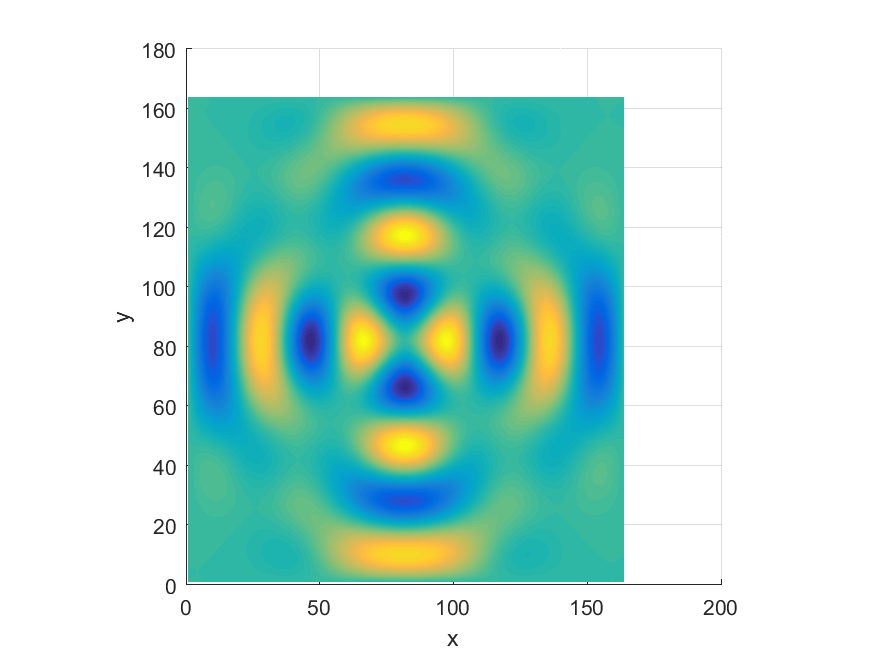
\includegraphics[width=6cm]{../Chapter_4/_Figs/Quadrupole_lateral_001_5point_160Hz_L10m_8000Fs.png}
	\caption{T=0.015s}
\end{subfigure}
\begin{subfigure}{0.3 \textwidth}
	\centering
	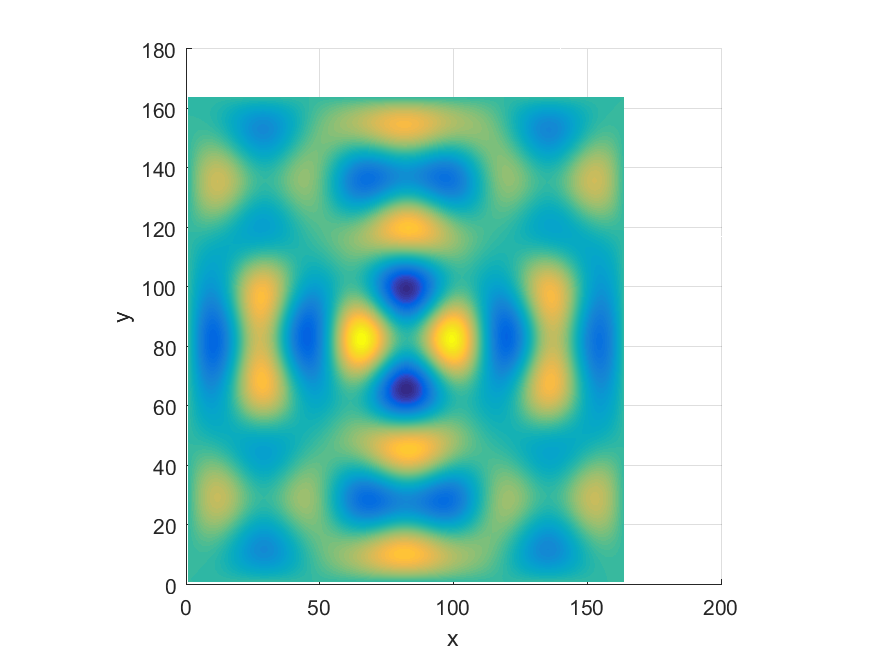
\includegraphics[width=6cm]{../Chapter_4/_Figs/Quadrupole05_lateral_5point_160Hz_L10m_8000Fs.png}
	\caption{T=0.3s}
\end{subfigure}
\begin{subfigure}{0.3 \textwidth}
	\centering
	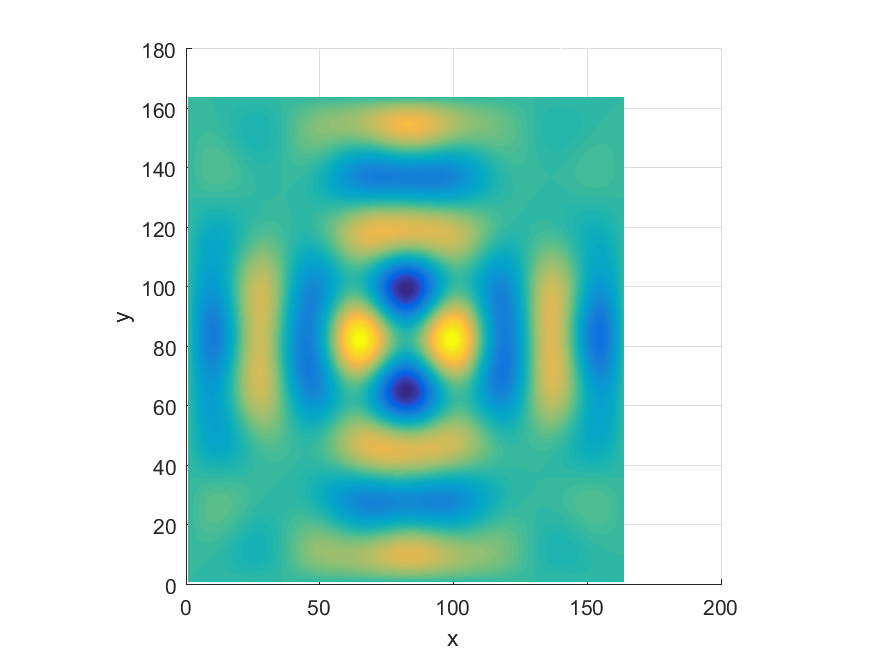
\includegraphics[width=6cm]{../Chapter_4/_Figs/Quadrupole1_lateral_5point_160Hz_L10m_8000Fs.png}
	\caption{T=1s}
\end{subfigure}
\label{figs:latquad}
\end{figure}


%%%%%%%%%%%% EDIT %%%%%%%%%%%%
%%%%%%%%%%%%%%%%%%%%%%%%%%%%%%%%%%%%%%%%%%%%%%%%%%%%%%%%%%
% Acoustics and Music Technology Final Project Latex Template
%
% CHAPTER 5 PAGE
%
% TOTAL EDITS REQUIRED: 1
%
% NOTE: NO NEED TO INCLUDE ANY FURTHER PREAMBLE IN THIS FILE
%%%%%%%%%%%%%%%%%%%%%%%%%%%%%%%%%%%%%%%%%%%%%%%%%%%%%%%%%%


%%%%%%%%%%%% EDIT %%%%%%%%%%%%
\chapter{Results and Conclusion}
\label{chapter5}
Through this chapter the efficiency and accuracy of the code will be analyzed and it will conclude by gathering all the results obtained in order to give clear and concise information about the simulation.
\section{Accuracy}
\label{chapter5:sec1}
\subsection{Non grid points}
\label{chapter5:sec1:ss1}
One important aspect when analysing the accuracy of the simulation is that of a correct behaviour when the source or the reciever do not lie at a grid point. It is necessary to analyse the performance at non-grid points as they might give important information that is neglected at the grid points. In order to retrieve information at non-grid points, it is necessary to perform an interpolation of the grid. To show the accuracy at non grid points, a simple approach was taken. If we consider a source and reciever to be lying at different grid points and we shift both by the same amount so that they do not lie at a grid point  the results recorded for the reciever at both instances must be the same. The results obtained at both instances for a reciever are shown in figure [ ] where it is also shown that the difference between them lies within...
\label{chapter5:sec2}
\subsection{Rotation}
\label{chapter5:sec1:ss2}
It is of importance in terms of accuracy analysis that the system preserves information under rotation. In the case of the monopole, rotation is not necessary as the pattern radiation is omnidirectional. Hence, the displacement of any arbitrary point $u$ at a distance $r$ with respect to the source, must be the same. This is illustrated on Figure $\ref{figs:DissMono}$ where we can see that the degree of difference between two points at the same distance is always below $5\cdot10^{-12}$ in the case of the 5 point scheme while in the 9 point scheme, the difference is always below$1.5\cdot10^{-11}$. It is important to note that the simulation times for both schemes are different and it we can see how the nine point scheme has a higher level of accuracy. Although both simulation have some degree of inaccuracy, we can see how the approximation performs an omnidirectional pattern to machine accuracy.\\
\begin{figure}[tb!]
\begin{subfigure}{0.5 \textwidth}
	\centering
	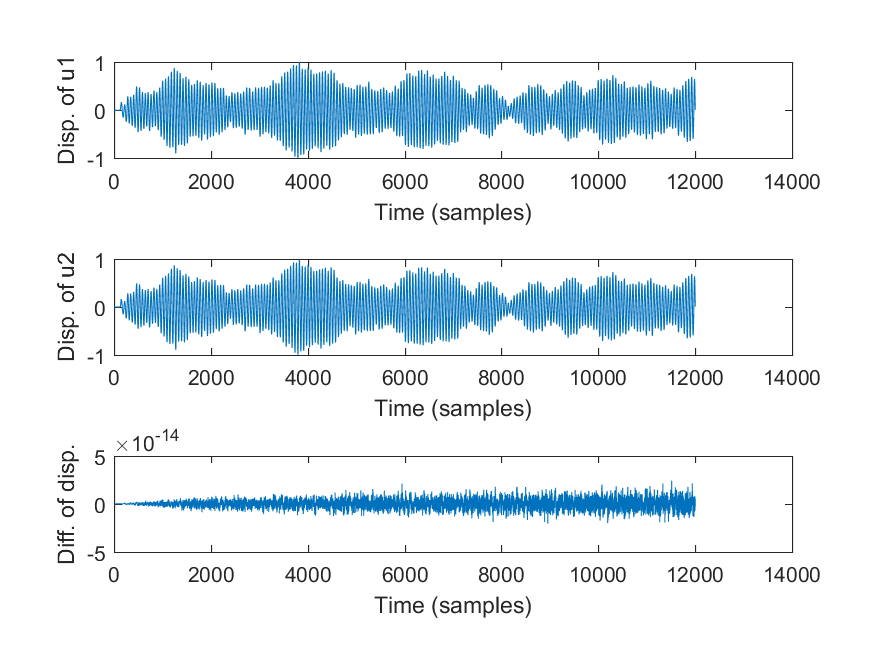
\includegraphics[width=8cm]{./Chapter_5/_Figs/RotationMonopole.png}
	\caption{Five point scheme}
\end{subfigure}
\begin{subfigure}{0.5 \textwidth}
	\centering
	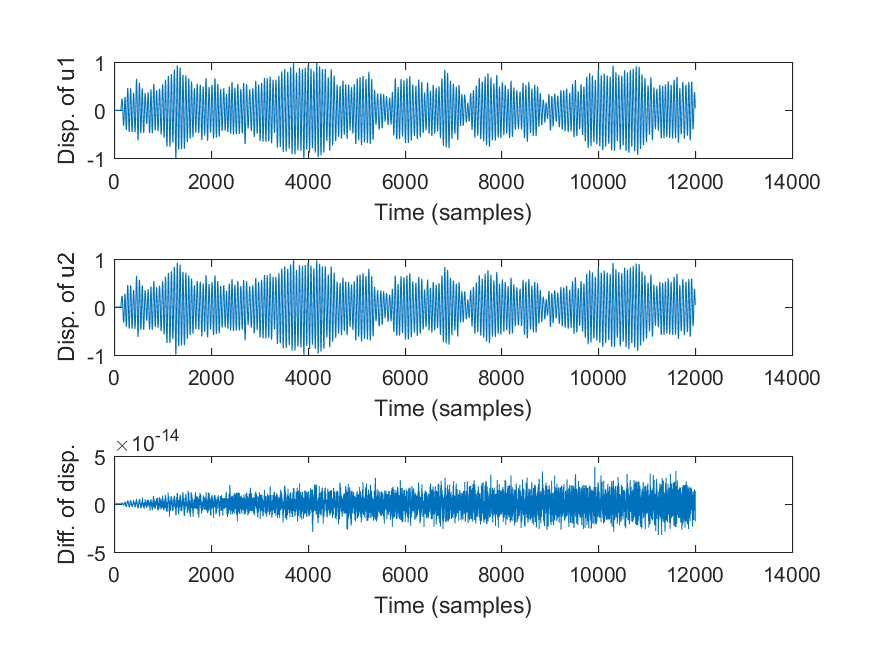
\includegraphics[width=8cm]{./Chapter_5/_Figs/RotationMonopole9.png}
	\caption{Nine point scheme}
\end{subfigure}
\caption{Top plots represent the Point u(20,50) displacement while bottom plots represent the difference with respect to point u(50,20) for the two different schemes.For Fs=12000, L=4 m where T= 1s  and $\alpha=0.65$.}
\label{figs:DissMono}
\end{figure}
Rotation of a dipole on the other hand, will produce diffrent radiation patterns and will excite different modes depending on the angle of rotation. Although, if we take in consideration a point reciever with respect to the source, if the source is rotated by an angle $\theta$, the rotation of the reciever by $\theta$ must achieve the same displacement. This is illustrated on Figure $\ref{figs:DissDi}$ where we can see how this invariance is preserved to a lower degree of accuracy with respect to the monopole but it is still below $1.5\cdot10^{-8}$ in the case of the five point scheme and $3\cdot10^{-8}$ in the case of the nine point scheme. Once again, considering the computation times are again 0.5 seconds for the five point scheme and 1s for the 9 point scheme, we can see how the later schem will produce a more accurate result under rotation.\\
\begin{figure}[h]
\begin{subfigure}{0.5 \textwidth}
	\centering
	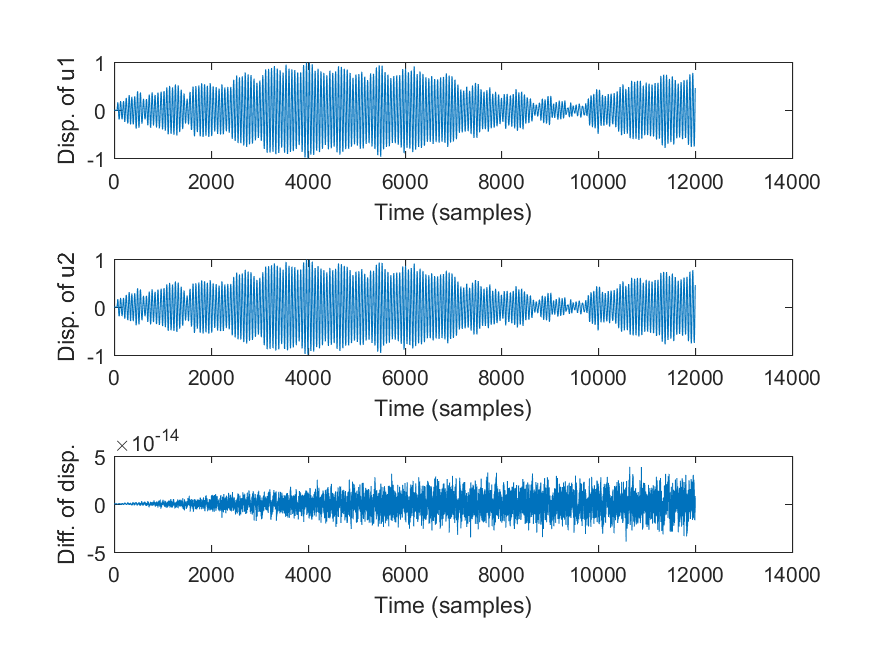
\includegraphics[width=8cm]{./Chapter_5/_Figs/RotationDipole.png}
	\caption{Five point scheme}
\end{subfigure}
\begin{subfigure}{0.5 \textwidth}
	\centering
	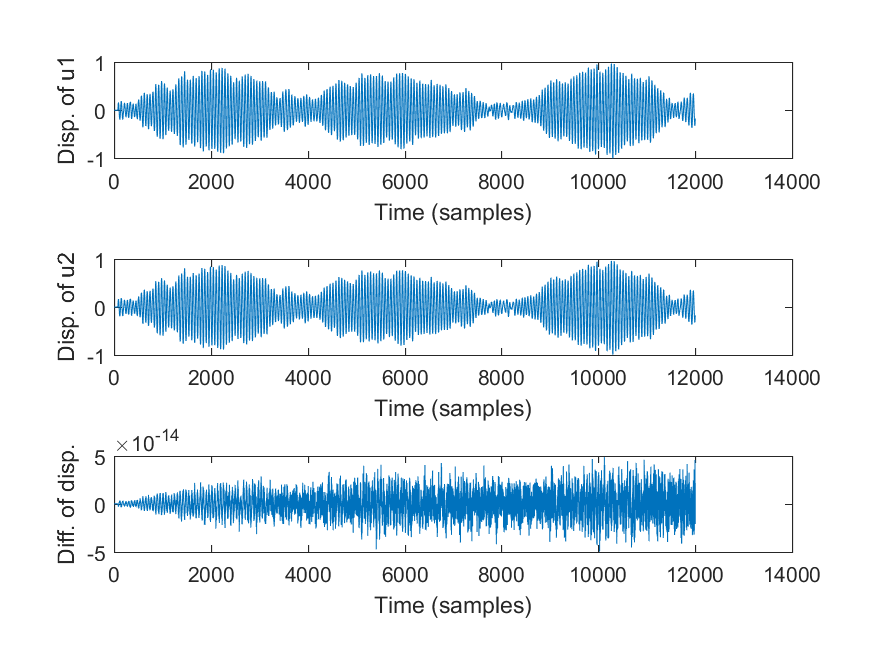
\includegraphics[width=8cm]{./Chapter_5/_Figs/RotationDipole9.png}
	\caption{Nine point scheme}
\end{subfigure}
\caption{Top plots represent the Point u(N/2,50) displacement while bottom plots represent the difference with respect to point u(50,N/2) for the two different schemes.For Fs=12000, L=4 m where  T= 1s  and $\alpha=0.65$.}
\label{figs:DissDi}
\end{figure}
\begin{figure*}
        \centering
        \begin{subfigure}[b]{0.475\textwidth}
            \centering
            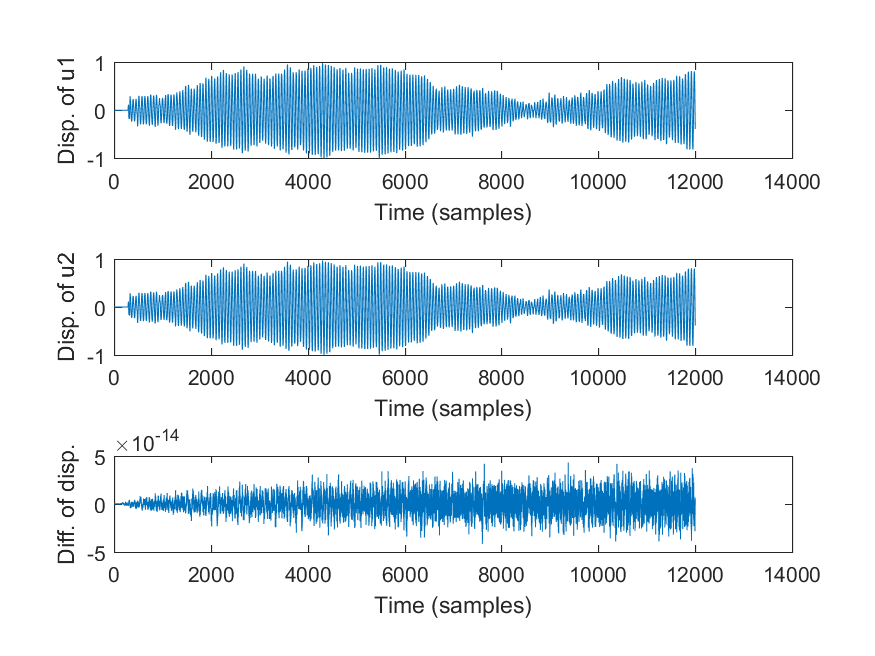
\includegraphics[width=\textwidth]{./Chapter_5/_Figs/RotationQuadrupoleLat.png}
            \caption[Network2]%
            {{\small Network 1}}    
            \label{fig:mean and std of net14}
        \end{subfigure}
        \hfill
        \begin{subfigure}[b]{0.475\textwidth}  
            \centering 
            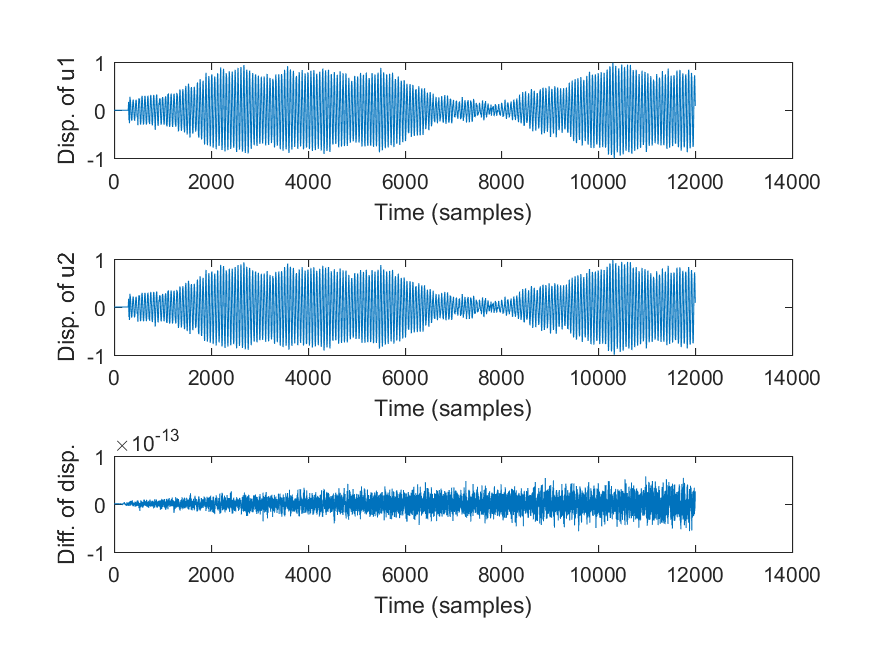
\includegraphics[width=\textwidth]{./Chapter_5/_Figs/RotationQuadrupoleLat9.png}
            \caption[]%
            {{\small Network 2}}    
            \label{fig:mean and std of net24}
        \end{subfigure}
        \vskip\baselineskip
        \begin{subfigure}[b]{0.475\textwidth}   
            \centering 
            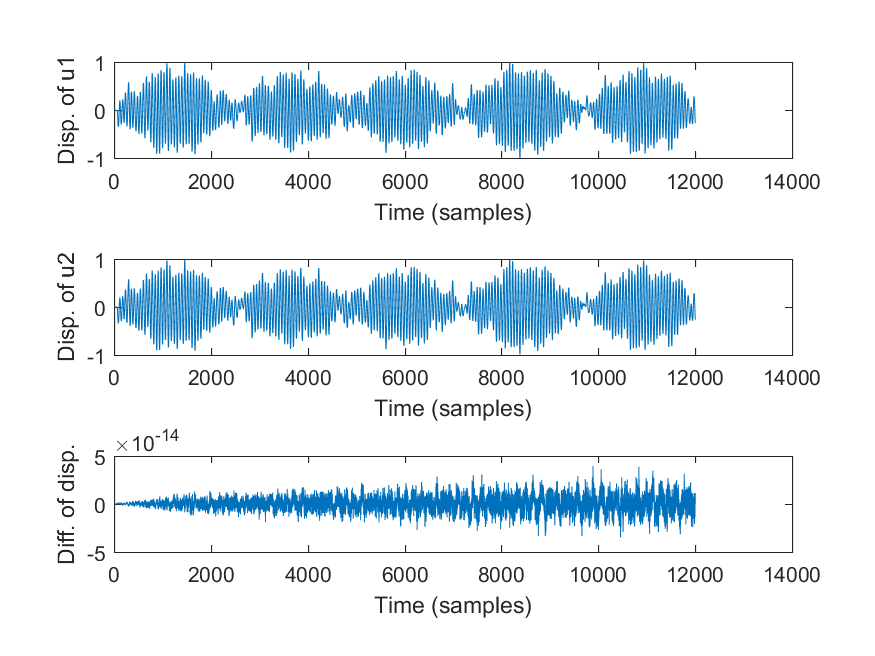
\includegraphics[width=\textwidth]{./Chapter_5/_Figs/RotationQuadrupoleLong.png}
            \caption[]%
            {{\small Network 3}}    
            \label{fig:mean and std of net34}
        \end{subfigure}
        \quad
        \begin{subfigure}[b]{0.475\textwidth}   
            \centering 
            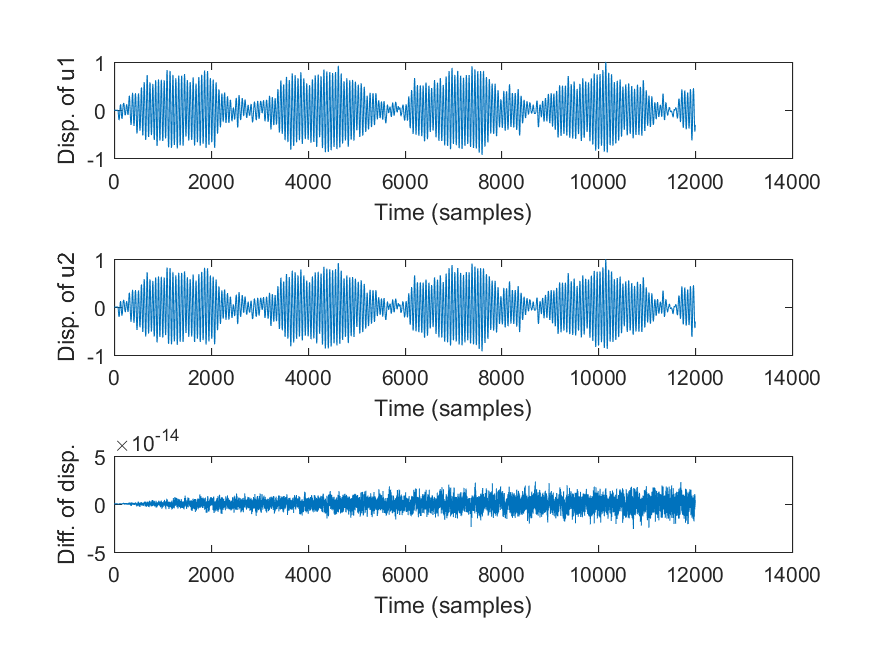
\includegraphics[width=\textwidth]{./Chapter_5/_Figs/RotationQuadrupoleLong9.png}
            \caption[]%
            {{\small Network 4}}    
            \label{fig:mean and std of net44}
        \end{subfigure}
        \caption[ The average and standard deviation of critical parameters ]
        {\small The average and standard deviation of critical parameters: Region R4} 
        \label{fig:mean and std of nets}
    \end{figure*}
%\label{figs:DissDi}
%\end{figure}
\section{Efficiency}
\label{chapter5:sec2}
One of the most important factors when producing these sort of simulations is that of time and memory usage. In order to optimize the results of the simulation, is necessary to find a balance in between the level of accuracy, memory usage and efficiency. The following table gives clear information about the time necessary to compute the simulation as well as the memory used to perform it. The simulations were produced by a standard computer (HP Compaq dc7800) and therefore can give an approximation to the results that will be obtained using an average PC nowadays.
\begin{table}[h]
	\centering
	\begin{adjustbox}{\textwidth}
	\small
	\begin{tabular}{|l|c|c|c|c|c|}
		\hline
		Fs & 5 Point Time(s)& 9 Point Time(s) & Memory (MB)& N. Points (5point)&N.Points (9point) \\
		\hline
		12000 & 2.15 & 5.958& 1100&98&122\\
		16000 & 4.569 & 12.686& 1105&131&163\\
		32000 & 39.487& 130.505 &1108 &263& 327\\
		44100 & 127.318 & 539.55 & 1114 & 363&451\\
		\hline
	\end{tabular}
	\end{adjustbox}
	\caption{Table of computing time and memory averages for monopole, dipole and quadrupole sources. For L=4 m, T=1 s and $\alpha=0.64$ ( 9 point Scheme), driven by a pure sine 			wave at 220Hz}
	\label{tab:Times}
\end{table}
As we can see in \ref{tab:Times} the computational times increase exponentially given an increasing sampling rate while the memory usage stays more or less the same. Therefore, it is worth noting that some degree of accuracy will be lost if optimization in terms of computing time is desired. 


%%%%%%%%%%%% EDIT %%%%%%%%%%%%

\renewcommand{\bibsection}{}
\chapter*{Riferimenti bibliografici}
\bibliography{refs}
\newpage

\renewcommand{\appendixtocname}{Appendici}
\renewcommand{\appendixpagename}{Appendici}
% \csname @openrightfalse\endcsname
\pagenumbering{gobble}
\begin{appendices}
\chapter{Appendice 1}
\label{Appendice:A}
Probabilmente ci sono un sacco di package non utilizzati ma così funziona tutto quindi non ho indagato oltre.

Inoltre su internet c'è un sacco di documentazione se ti servisse.
\chapter{Appendice B}
\label{Appendice:B}
Appendice B se serve

\chapter{Embed di interi PDF}
\label{Appendice:C}
Se ti serve puoi fare embed di PDF interi con pdfpage, scegliendo anche le pagine (o mettendo - se le vuoi tutte):

\includepdf[pages=1]{pdf/sample.pdf}
\end{appendices}

\newpage~\newpage
\chapter*{Ringraziamenti}
Grazie a tutti
\end{document}